

% -------------------------------------------------------------------------
% Title

\title{Article template}

\author{Spencer Woody\footnote{The University of Texas at Austin,
    Department of Statistics and Data Science. Email:
    \texttt{spencer.woody@utexas.edu}}}

\date{\today}

% -------------------------------------------------------------------------
%%
%% PREAMBLE
%%

% Page format
\documentclass[10pt]{article} % 10 pt might be a bit small
\usepackage[margin=1.25in]{geometry} % Set the margins

% Fonts
\usepackage{mathpazo} % Palatino for main and math text
\usepackage{inconsolata} % Inconsolata fixed width font

% Basics
\usepackage{graphicx} % including images
\usepackage{amsmath} 
\usepackage{amssymb}
\usepackage{subcaption}

% Bibliography format
\usepackage[round]{natbib} 
\bibliographystyle{plainnat}

% For using Computer Modern version of blackboard symbols
\AtBeginDocument{
  \DeclareSymbolFont{AMSb}{U}{msb}{m}{n}
  \DeclareSymbolFontAlphabet{\mathbb}{AMSb}}

% -------------------------------------------------------------------------
%%
%% END DOCUMENT
%%
% -------------------------------------------------------------------------

\begin{document}

\maketitle

% -------------------------------------------------------------------------
% Abstract

\begin{abstract}
  Lorem ipsum dolor sit amet, consectetur adipiscing elit. Nullam
  maximus tristique lorem, et dignissim dolor fermentum a. Aenean
  hendrerit convallis mauris nec mattis. Nunc imperdiet malesuada
  tellus. Sed pulvinar libero ac tortor condimentum, a fringilla eros
  tincidunt. In ut dolor eu dolor rhoncus blandit. Sed placerat
  viverra elementum. Pellentesque tortor mauris, sollicitudin ut
  rutrum id, efficitur eu magna. Donec sit amet libero non nulla
  blandit congue. Proin ultrices id metus a tristique. Interdum et
  malesuada fames ac ante ipsum primis in faucibus. Suspendisse
  interdum pretium varius. Proin sit amet risus vitae enim mattis
  venenatis. Phasellus bibendum ultricies risus, non semper arcu
  tincidunt id. Nullam dictum enim ac felis vestibulum elementum eu a
  tortor. Sed at diam faucibus, accumsan lectus vitae, condimentum
  ante.
\end{abstract}

% -------------------------------------------------------------------------
% Main body

% \pagebreak


\section{Introduction}
\label{sec:introduction}

\cite{einstein} showed mass-energy equivalence
%
\begin{align}
  \label{eq:1}
  E &= mc^2,
\end{align}
%
for speed of light $c= 2.99792458 \times 10^{8}$ m/s.

\begin{figure}[!h]
  \centering
  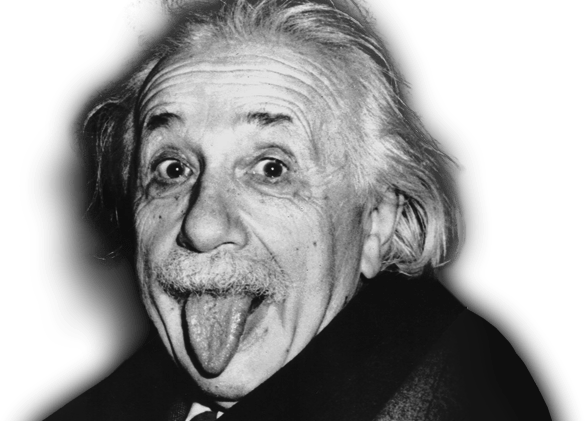
\includegraphics[scale=0.25]{fig/einstein.png}
  \caption{Albert Einstein}
  \label{fig:einstein}
\end{figure}

%%% Local Variables:
%%% mode: latex
%%% TeX-master: "../main"
%%% End:


% -------------------------------------------------------------------------
% Bibliography
\bibliography{main}

% -------------------------------------------------------------------------
%%
%% END DOCUMENT
%%
% -------------------------------------------------------------------------


\end{document}